\begin{center}
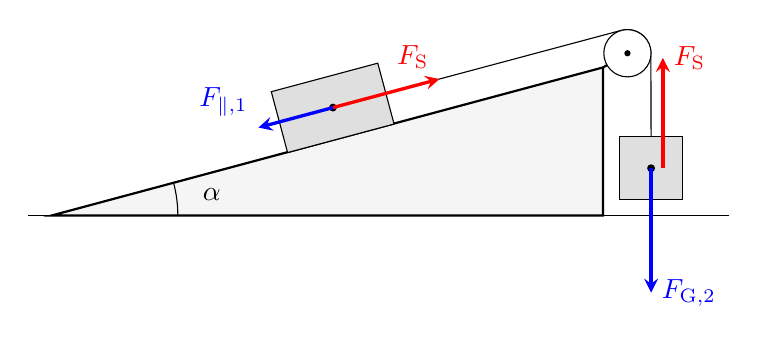
\begin{tikzpicture}[>=stealth]
 \draw[thick, fill=gray!8] (0,0) -- (7.00,0) -- (7.00,1.88) -- cycle;
 \draw (-0.3,0) -- (8.60,0);
 \draw (1.6,0) arc (0:15:1.6);
 \node at (2.03,0.27) {$\alpha$};
 \begin{scope}[shift={(3.67,0.98)}, rotate=15]
  \draw[fill=gray!25] (-0.7,0) rectangle (0.7,0.8);
 \end{scope}
 \draw[thick] (7.00,1.88) -- (7.31,2.06);
 \draw (4.24,1.55) -- (7.23,2.35) arc (105:0:0.3) -- (7.61,1.0);
 \draw[fill=white] (7.31,2.06) circle (0.3);
 \fill (7.31,2.06) circle (0.04);
 \draw[fill=gray!25] (7.21,0.2) rectangle (8.01,1.0);
 \fill (3.57,1.37) circle (0.05);
 \draw[->, very thick, red] (3.57,1.37) -- ++(15:1.40) node[anchor=south east] {$F_\mathrm{S}$};
 \draw[->, very thick, blue] (3.57,1.37) -- ++(195:0.98) node[anchor=south east] {$F_{\parallel,1}$};
 \fill (7.61,0.6) circle (0.05);
 \draw[->, very thick, red] (7.76,0.6) -- ++(0,1.40) node[right] {$F_\mathrm{S}$};
 \draw[->, very thick, blue] (7.61,0.6) -- ++(0,-1.58) node[right] {$F_\mathrm{G,2}$};
\end{tikzpicture}
\end{center}

Die Reibung wird vernachlässigt. Längs des Seils wirken auf das System der beiden Kisten nur die Hangabtriebskraft $m_1\,g\sin\alpha$ auf die erste Kiste und die Gewichtskraft $m_2\,g$ der hängenden Kiste. Die Seilkraft $F_\mathrm{S}$ ist eine innere Kraft.
\begin{abcliste}
\abc Gleichgewicht herrscht, wenn sich die beiden Kräfte aufheben: $m_1\,g\sin\alpha = m_2\,g$, also
\begin{align}
 m_1 &= \mGlF = \frac{\mZw}{\sin\left(\wiO\right)} = \mGl \approx \result{\mGlP{0}{2}}
\end{align}

\abc Mit $m_1 = \mEiO$ ist die Hangabtriebskraft kleiner als $m_2\,g$; die hängende Kiste sinkt, die erste Kiste wird hangaufwärts gezogen. Das Aktionsprinzip für beide Kisten zusammen gibt
\begin{align}
 \left(m_1+m_2\right)a &= m_2\,g - m_1\,g\sin\alpha \\
 a &= \aKiF \\
   &= \frac{\mZw-\mEi\cdot\sin\left(\wiO\right)}{\mEi+\mZw}\cdot\gE \\
   &= \aKi \approx \result{\aKiP{0}{2}}
\end{align}
$m_2$ beschleunigt nach unten, $m_1$ hangaufwärts.

\abc Für die hängende Kiste allein gilt $m_2\,g - F_\mathrm{S} = m_2\,a$, also
\begin{align}
 F_\mathrm{S} &= \FSeF = \mZw\cdot\left(\gE-\aKi\right) = \FSe \approx \result{\FSeP{0}{2}}
\end{align}
Das leichte Seil zieht an beiden Kisten mit derselben Kraft. Kontrolle mit der ersten Kiste, $F_\mathrm{S} - m_1\,g\sin\alpha = m_1\,a$:
\begin{align}
 F_\mathrm{S} &= \FScF = \FSc
\end{align}
\end{abcliste}
